\subsection{Egyptians: Astronomy as a tool for agriculture and belief}
\initial{S}ome celestial bodies like the Sun and the Moon were documented already five thousand years ago!
Indeed, astronomy being a science of observation, Egyptians did not need more than looking into the sky to discover bodies.
Although more difficult to observe, five planets could already be seen by the naked eye due to their size and brightness:
Mercury, Venus, Jupiter, Mars and Saturn.
However, we had to wait until Copernicus in 1543 to finally recognize Mars as a planet!

Egyptians' main interests for the sky were mainly agricultural and religious.
The Egyptians studied the positions and alignments of stars to build pyramids, and the size of the Moon determined periods of harvest.
For the same purpose, they already used the 365 days calendar.
Religion also played a great part in ancient astronomy as gods were viewed as constellations.
\cite{Egyptians}

\begin{center}
	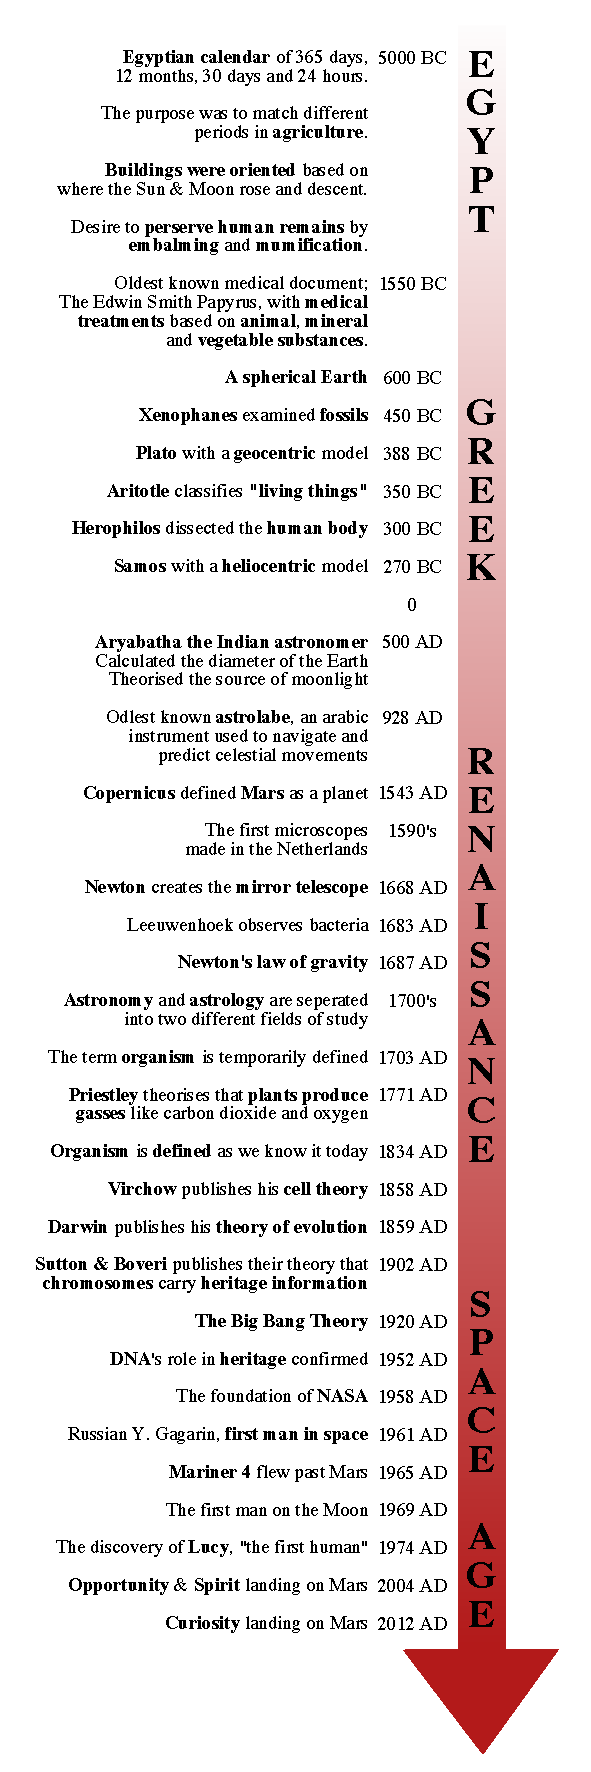
\includegraphics[width=0.475\textwidth]{timeline.pdf}
\end{center}

\subsection{Ancient Greeks, Arabs and Indians: The age of theories}
\initial{I}t is not until the Greek period, starting around 600 BC, that humanity tried to really understand and explain astronomy. 
To start with, they thought that Earth was flat, surrounded by water and that the stars were emerging from it.
Plato, followed by Ptolemy and Aristotle, were the pioneers of the geocentric model: the Sun, the Moon and the planets move in harmony around Earth, the center.

A hundred years later, another Greek, Samos, proposed the opposite theory called heliocentrism: the Sun is now the center of the Universe.
How fascinating to see how much they actually discovered at that time!  
Without tools such as the telescope, without communication within the community of scientists around the world, Greeks, Arabs and Indians still made great assumptions on how our universe worked. 
For example, the Indian astronomer, Aryabatha, not noly did he have some ideas about gravitation but also that the movement of planets around the Sun were elliptical and not circular.
He even understood that the light coming from the Moon was refracted sunlight, and not the Moon itself glowing in the dark sky.
One might wonder, how much we would know in the present time if ancient astronomers had the tools of communication we have today?
\cite{GreekAstro}
\cite{Aryabatha}

\subsection{European Renaissance: The age of reason and experimentation}
\initial{W}ith new technologies and the rediscoveries and translations of ancient Greek texts, the scientists of the renaissance period, were able to make very accurate calculations of the stars and planets.
Intellectuals in this period defined and proved the basic of astronomy as we know it today.  
Scientists such as Copernicus, Galileo and Kepler defined the heliocentric model to the world. 
It was definitely the age of reason and scientific truth. 
We can notice for example, that it is during that time that astronomy and astrology were separated into two different fields. 
Technologies and communications became more advanced and enabled physicists to search deeper and with more accuracy. 
In 1609, the Italian astronomer Galileo was one of the first people to point a telescope skyward. 
Although that telescope was far from perfected, Galileo was able to see that the Moon's surface was made of craters and mountains instead of being smooth as we thought.
As their view expanded dramatically by the telescope, astronomers were also able to discover many stars and to calculate stellar distances.
\cite{GalileoTelescope}

\subsection{Space Age: Not only studying Astronomy but also Exploring!}
\initial{I}n 1957, The Soviet Union launched Sputnik, the first spacecraft placed in orbit around Earth, marking the beginning of space exploration.
We are not only interested in studying, but also of exploring.
The space age represents an effort that is as scientific as it is political.
Indeed, this happened during the Cold War when the Soviet Union and the USA raced in different domains, including astronomy.

This space race focused particularly on discovery by humans and machines in the solar system and the development of technology.
Rockets were one of the most obvious forms of space age technology.
The creation of NASA, followed by the Apollo program was definitely highlights of the space age.
The most famous of the Apollo aircrafts was Apollo 11, carrying commander Neil Armstrong and his fellow astronauts Michael Collins and Edwin 'Buzz' Aldrin to the Moon.
On that mission, Armstrong and Aldrin were the first humans to land and walk on the Moon.
"That's one small step for a man, one giant leap for mankind."
\cite{SpaceAge}